\chapter{DNS}

O DNS, Domain Name System, é o serviço responsável por receber um nome, como
exemplo o nome de um site “www.unb.br”, e retornar o endereço IP desse
nome.

Para o estudo da aplicação DNS foi feito um programa em ruby, que recebe como
argumento o nome a ser enviado para o DNS, e opcionalmente o IP de um DNS, caso
o IP do DNS não seja transmitido será usado o DNS padrão. A figura~\ref{fig:ruby_get_dns}
mostra o código do programa em ruby.

\begin{figure}[h]
  \centering
  \includegraphics[width=0.9\textwidth]{figuras/ruby_get_dns.eps}
  \caption{Código do programa que faz requisição ao DNS}
  \label{fig:ruby_get_dns}
\end{figure}

O programa foi executado utilizando o DNS padrão e o DNS 8.8.8.8, os tópicos
seguintes descrevem cada uma das execuções

\section{DNS Padrão}

O programa em ruby foi executado através da seguinte linha de comando:
“./get{\_}dns.rb www.unb.br”. O resultado da execução é mostrado na
figura~\ref{fig:ruby_default_dns}. Onde observa-se que o DNS padrão possui
o IP “192.168.2.1”, e o DNS retorna o IP “164.41.101.33” para nome “www.unb.br”

\begin{figure}[h]
  \centering
  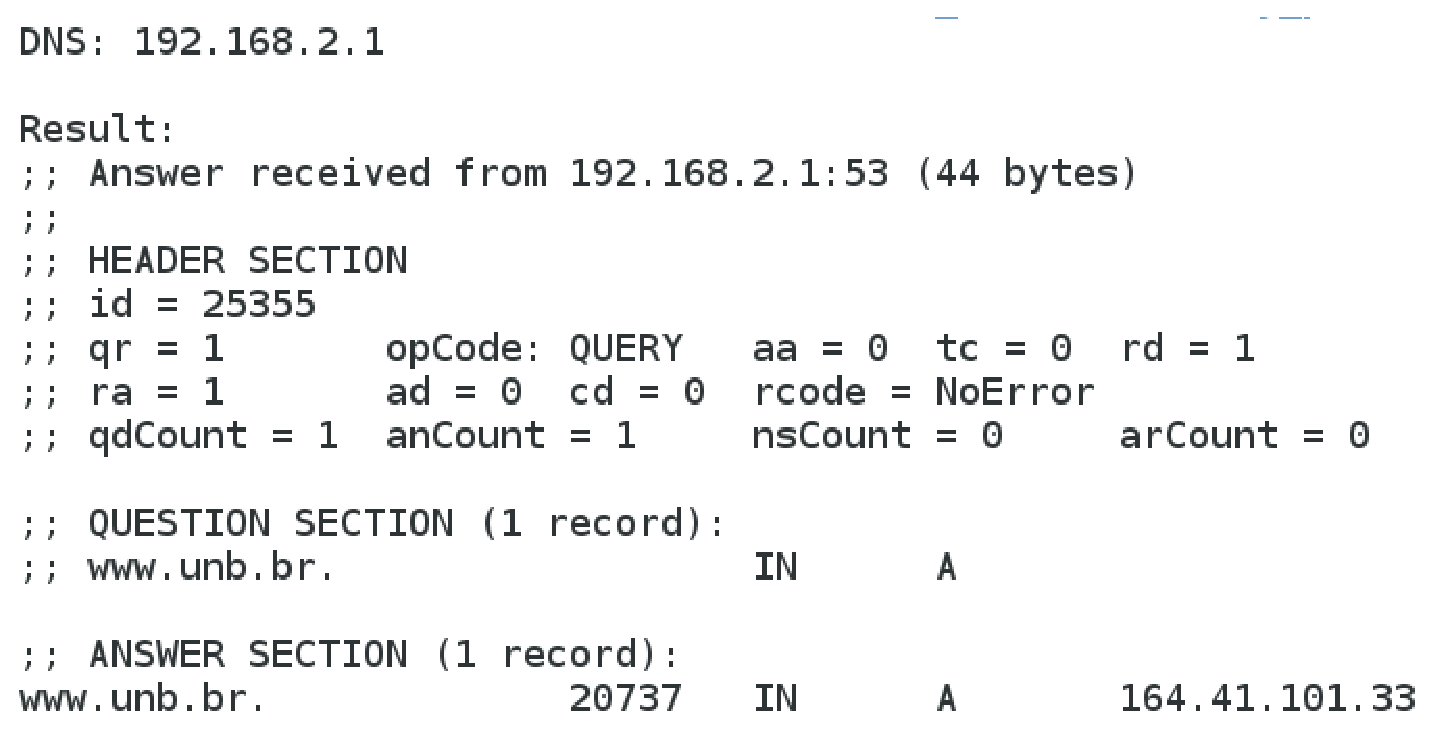
\includegraphics[width=0.9\textwidth]{figuras/ruby_default_dns.eps}
  \caption{Código do programa que faz requisição ao DNS}
  \label{fig:ruby_default_dns}
\end{figure}

O acompanhamento dos pacotes na rede foi realizado através do programa
wireshark, onde observa-se que os pacotes são enviados pela rede utilizando
os protocolos UDP e o IP, a figura~\ref{fig:wireshark_dns} mostra a
execução do programa wireshark, e a figura~\ref{fig:wireshark_dns_protocol} mostra
os protocolos utilizados.

\begin{figure}[h]
  \centering
  \includegraphics[width=0.9\textwidth]{figuras/wireshark_dns.esp}
  \caption{Execução do programa wireshark para o DNS padrão}
  \label{fig:wireshark_dns}
\end{figure}

\begin{figure}[h]
  \centering
  \includegraphics[width=0.9\textwidth]{figuras/wireshark_dns_protocol.eps}
  \caption{Execução do programa wireshark para o DNS padrão mostrando os protocolos}
  \label{fig:wireshark_dns_protocol}
\end{figure}


\section{Outro DNS}

O programa em ruby foi executado através da seguinte linha de comando:
“./get{\_}dns.rb www.unb.br 8.8.8.8”. O resultado da execução é mostrado na
figura~\ref{fig:ruby_default_dns}. Onde observa-se que o DNS possui
o IP “8.8.8.8”, e o DNS retorna o IP “164.41.101.33” para nome “www.unb.br”

\begin{figure}[h]
  \centering
  \includegraphics[width=0.9\textwidth]{figuras/ruby_other_dns.eps}
  \caption{Código do programa que faz requisição ao DNS}
  \label{fig:ruby_other_dns}
\end{figure}

O acompanhamento dos pacotes na rede foi realizado através do programa
wireshark, onde observa-se que os pacotes são enviados pela rede utilizando
os protocolos UDP e o IP, a figura~\ref{fig:wireshark_other_dns} mostra a
execução do programa wireshark, e a figura~\ref{fig:wireshark_other_dns_protocol} mostra
os protocolos utilizados.

\begin{figure}[h]
  \centering
  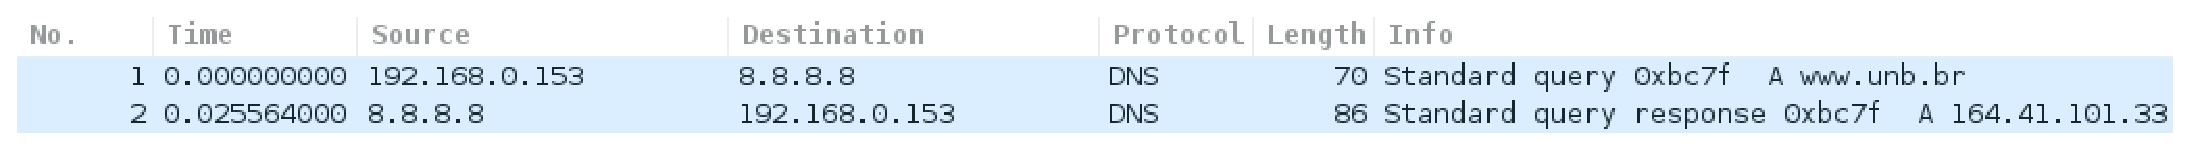
\includegraphics[width=0.9\textwidth]{figuras/wireshark_other_dns.eps}
  \caption{Execução do programa wireshark para o DNS padrão}
  \label{fig:wireshark_other_dns}
\end{figure}

\begin{figure}[h]
  \centering
  \includegraphics[width=0.9\textwidth]{figuras/wireshark_other_dns_protocol.eps}
  \caption{Execução do programa wireshark para o DNS padrão mostrando os protocolos}
  \label{fig:wireshark_other_dns_protocol}
\end{figure}
